\documentclass[12pt]{article}
\usepackage{amsmath}    % For advanced math formatting
\usepackage{amssymb}    % For mathematical symbols
\usepackage{graphicx}   % For including graphics
\usepackage{booktabs}   % For better table formatting
\usepackage{geometry}   % For page margins
\usepackage{setspace}   % For line spacing
\usepackage{hyperref}   % For hyperlinks
\usepackage{caption}    % For better caption control
\usepackage{subcaption} % For subfigures
\usepackage{float}      % For better figure placement
\usepackage{mathtools}  % For additional math tools
\usepackage{pgfplots} 
\pgfplotsset{compat=1.18}
\usepgfplotslibrary{statistics}

% Page setup
\geometry{a4paper, margin=1in}
\setlength{\parindent}{0.5in}
\setlength{\parskip}{0.5em}
\onehalfspacing
\usepackage{graphicx} % Required for inserting images

\title{Multivar Model Project BM and BM}
\author{ }
\date{April 2025}

\begin{document}

\maketitle

\section{Problem Restatement}
Charitable organizations play a crucial role in addressing systemic global issues, from poverty and disease to social justice and animal rights. However, not all are equally effective at turning donations into real-world impact. Donors today face a growing challenge: determining which of the numerous available nonprofits use their financial resources most efficiently and sustainably. While some charity review organizations like GiveWell attempt to measure nonprofit effectiveness, there remains no standardized or transparent system for evaluating financial performance and effectiveness using publicly available data. Our task was to design a mathematical model that objectively ranks nonprofit organizations based on key financial indicators derived from IRS Form 990s. By focusing on reach, scalability, cost-effectiveness, and financial sustainability, our model seeks to offer an accessible and data-driven tool for assessing charitable financial effectiveness.

\section{Introduction}

Charitable organizations are vital actors in modern society, addressing a wide range of systemic issues such as poverty, education inequality, healthcare access, and environmental degradation. These organizations function by mobilizing resources – most often in the form of financial donations, volunteer labor, or material goods – from individuals or institutions and reallocating them to areas of need, typically without direct compensation or market exchange. The core motivation behind this process is frequently rooted in altruism: the selfless concern for the well-being of others. Unlike profit-driven enterprises, charities operate based on values that prioritize social benefit over financial return, making their behavior and impact uniquely suited for study through models that incorporate ethical and behavioral dimensions alongside economic efficiency. \\

However, not all charities are created equal. Like large corporations, nonprofit organizations have operating costs and overhead expenses that can diminish the impact of civilian donations. Furthermore, charities use their financial resources in vastly different ways, achieving varying degrees of efficiency and societal benefit. To help donors navigate these differences, a range of organizations have emerged that specialize in evaluating nonprofits' effectiveness, most notably the San Francisco-based GiveWell and New Jersey-based Charity Navigator.\\

Organizations like GiveWell typically assess charities through two main dimensions: financial effectiveness – how sustainably and efficiently they manage and use their funds; and utilitarian impact – the overall good they create through their interventions. While measuring utilitarian impact involves subjective judgments (such as valuing current versus future lives, or comparing human and animal welfare), financial effectiveness is more objectively measurable through publicly available data. \\

Despite this, there is currently no standardized system or model that efficiently calculates financial effectiveness based on nonprofit financial filings. To help fill this gap, we developed a mathematical model aimed at objectively evaluating and ranking charities' financial performance and effectiveness. Our model emphasizes four primary factors: the organization's reach within its focus area, the scalability of the problem it addresses, its cost-effectiveness, and its overall financial sustainability. This model could potentially be utilized by organizations like BindWell and Charity Navigator as a factor within their analyses, as well as by the average person to, among other factors, inform them how effectively their donations are used. 

\section{Assumptions}

\section*{Model Assumptions}

\subsection*{Core Definition}
\begin{itemize}
    \item We define altruistic effectiveness as a charity's ability to sustainably and efficiently operate in service of its mission, with strong governance and transparency. This includes financial health, administrative efficiency, structural scalability, and robust internal controls, rather than direct quantification of moral or utilitarian "impact" (such as QALYs or lives saved).
\end{itemize}

\subsection*{Scope and Applicability}
\begin{itemize}
    \item Our model does not attempt to assess what causes are most ethical or impactful. Instead, we evaluate how effectively an organization is structured and funded to carry out its mission, regardless of cause area.
    
    \item While our model is designed to be applicable across nonprofit sectors, we acknowledge that certain metrics may need sector-specific calibration for optimal performance.
\end{itemize}

\subsection*{Data and Transparency}
\begin{itemize}
    \item We assume that IRS Form 990s are a reliable and standardized source of financial information across nonprofits. While not perfect, they represent the most comprehensive and standardized financial reporting framework available for comparative analysis.
    
    \item We assume that data reported in Form 990s (e.g., revenue, expenses, grants, compensation) are accurate and suitable for comparative analysis, with appropriate safeguards against data quality issues affecting the final score.
    
    \item We assume that missing or incomplete data in Form 990s can be reasonably handled through our normalization and weighting processes.
\end{itemize}

\subsection*{Financial and Operational Metrics}
\begin{itemize}
    \item We assume that a higher ratio of program service expenses to total expenses (vs. admin/fundraising) reflects a stronger alignment with mission-oriented work, and thus higher operational effectiveness. We recognize that some administrative and fundraising expenses are necessary for organizational health and growth.
    
    \item We incorporate multiple dimensions of sustainability, including revenue diversification, expense management, and reserve adequacy. These are weighted according to their relative importance in maintaining long-term organizational viability.
    
    \item While we acknowledge potential correlations between different financial metrics, we treat them as independent components in our model, allowing for a more granular assessment of organizational effectiveness.
\end{itemize}

\subsection*{Scalability and Longevity}
\begin{itemize}
    \item While we do not model scalability in terms of intervention outcomes, we assume that organizations with lower marginal administrative costs and stable operating budgets are more capable of scaling operations without compromising structural integrity.
    
    \item We assume that the financial metrics used in our model provide a stable basis for comparison across different time periods, with appropriate normalization to account for economic conditions and organizational life cycles.
\end{itemize}

\subsection*{Model Design and Application}
\begin{itemize}
    \item The weights assigned to each component in our model reflect both industry best practices and the relative importance of each factor in determining overall organizational effectiveness. These weights are subject to validation and potential adjustment based on empirical evidence.
    
    \item We envision this model serving as a first-pass filter in a multi-stage evaluation process, helping to identify organizations that meet basic structural and financial criteria before more resource-intensive impact assessments are conducted.
    
    \item Since we are not modeling direct impact or long-term outcomes, we do not apply a temporal discount rate in this version of the model.
    
    \item Unlike in impact-based models, we do not differentiate effectiveness based on beneficiary species or sentience. The focus is entirely on organizational structure and financial operations.
\end{itemize}

\section{Model Building}

The Altruistic Effectiveness Metric (AEM) was developed through a rigorous mathematical framework that combines multiple financial indicators into a single, normalized score. The model's foundation lies in the principle that a charity's effectiveness can be quantified through a weighted combination of key financial metrics, each carefully normalized and adjusted for statistical robustness.

\subsection{Mathematical Framework}

The core AEM score is calculated as a weighted sum of six normalized components:

\begin{equation}
    \text{AEM} = \sum_{i=1}^{6} w_i \cdot f_i(x_i)
\end{equation}

where $w_i$ represents the weight of each component and $f_i(x_i)$ is the normalized score for each metric. The weights are carefully calibrated based on both base importance and information content:

\begin{equation}
    w_i = \frac{w_i^{\text{base}} + w_i^{\text{entropy}}}{2}
\end{equation}

\subsection{Multi-Dimensional Normalization}

To ensure comparability across organizations while accounting for metric correlations, we employ a sophisticated multi-dimensional normalization approach based on Mahalanobis distance principles:

\begin{equation}
    \mathbf{z} = \frac{\mathbf{x} - \mathbf{\mu}}{\mathbf{\sigma}}
\end{equation}

where $\mathbf{x}$ is the vector of raw metrics, $\mathbf{\mu}$ is the mean vector, and $\mathbf{\sigma}$ is the standard deviation vector. This z-score normalization is then transformed into the unit interval using a sigmoid function:

\begin{equation}
    f(\mathbf{z}) = \frac{1}{1 + e^{-\beta(\mathbf{z} - \alpha)}}
\end{equation}

This approach provides several advantages:
\begin{itemize}
    \item Accounts for correlations between metrics
    \item Maintains relative distances between organizations
    \item Ensures bounded output between 0 and 1
    \item Provides smooth transitions between score ranges
\end{itemize}

\subsection{Weighting Methodology} % Explains another key calculation step
The weights $w_i$ in Equation \ref{eq:aem_core} determine the relative importance of each component. We use a hybrid approach combining expert judgment (base weights) and data-driven insights (entropy weights):
\begin{enumerate}
    \item \textbf{Base Weights ($w_i^{\text{base}}$):} Initial weights are assigned based on perceived importance in nonprofit evaluation literature and best practices (see Table \ref{tab:metrics_params}).
    
    \item \textbf{Entropy Weights ($w_i^{\text{entropy}}$):} To account for the information content or discriminative power of each metric within the dataset, we calculate weights based on Shannon entropy. First, normalized scores $s_i$ are treated as probabilities $p_i(s) = (s_i + \epsilon) / \sum (s_j + \epsilon)$, where $\epsilon=10^{-10}$ ensures numerical stability. The entropy $H_i$ for each metric across all organizations is calculated. Metrics with lower entropy (more variation, better discrimination) receive higher weights:
    \begin{equation} \label{eq:entropy_weight}
        w_i^{\text{entropy}} = \frac{H_{\max} - H_i + \epsilon}{\sum_{j=1}^{6} (H_{\max} - H_j + \epsilon)}
\end{equation}
    where $H_{\max}$ is the maximum entropy across all metrics. This formulation ensures that metrics with lower entropy (more information content) receive higher weights, as they provide more discriminative power in distinguishing between organizations.

    \item \textbf{Final Weights ($w_i$):} The final weight is the average of the base and entropy weights, normalized to sum to 1:
    \begin{equation} \label{eq:final_weight}
        w_i = \frac{w_i^{\text{base}} + w_i^{\text{entropy}}}{2}, \quad \text{then re-normalize so } \sum w_i = 1
\end{equation}
\end{enumerate}

This weighting methodology ensures that:
\begin{itemize}
    \item Each component's importance is based on both expert judgment and data-driven insights
    \item Metrics with more discriminative power (lower entropy) receive higher weights
    \item The final weights maintain a balance between theoretical importance and empirical significance
    \item Numerical stability is maintained through the use of $\epsilon$ and proper normalization
\end{itemize}

\subsection{Multi-Dimensional Normalization}

The multi-dimensional normalization process includes several safeguards:

\begin{equation}
    \mathbf{z} = 
    \begin{cases}
    \text{clip}\left(\frac{\mathbf{x} - \mathbf{\mu}}{\mathbf{\sigma}}, -3, 3\right) & \text{if } \mathbf{\sigma} \neq 0 \\
    0.5 & \text{otherwise}
    \end{cases}
\end{equation}

This ensures that:
\begin{itemize}
    \item Extreme values are clipped to prevent distortion
    \item Identical values result in neutral scores
    \item Zero standard deviation is handled gracefully
\end{itemize}

\subsection{Policy Evaluation}

The transparency component evaluates four key policies with equal weights:

\begin{table}[h]
\centering
\begin{tabular}{|l|c|}
\hline
\textbf{Policy} & \textbf{Weight} \\
\hline
Conflict of Interest & 0.25 \\
Whistleblower & 0.25 \\
Document Retention & 0.25 \\
Compensation Review & 0.25 \\
\hline
\end{tabular}
\caption{Policy Weights for Transparency Evaluation}
\label{tab:policy_weights}
\end{table}

The transparency score is calculated as:

\begin{equation}
    \text{Transparency} = \frac{1}{4}\sum_{k=1}^{4} \mu_k(p_k)
\end{equation}

where $\mu_k(p_k)$ is 1 if policy $k$ is implemented and 0 otherwise.

\subsection{Component Metrics}

The model incorporates six key metrics, each with specific normalization parameters:

\begin{table}[h]
\centering
\begin{tabular}{|l|c|c|}
\hline
\textbf{Metric} & \textbf{Base Weight} & \textbf{Normalization Parameters} \\
\hline
Program Expense Ratio & 0.30 & Ideal = 0.6, $\beta = 3$ \\
Fundraising Efficiency & 0.20 & Log scale, Ideal = 0.8, $\beta = 3$ \\
Revenue Sustainability & 0.15 & Ideal = 0.5, $\beta = 3$ \\
Net Surplus Margin & 0.15 & Ideal = 0.05, $\beta = 3$ \\
Executive Pay Reasonableness & 0.10 & Ideal = 0.015, $\beta = 3$ \\
Transparency & 0.10 & Binary, $\beta = 3$ \\
\hline
\end{tabular}
\caption{Component Metrics and Their Parameters}
\label{tab:metrics}
\end{table}

\subsection{Normalization Functions}

Each metric is normalized using a sigmoid function with specific parameters:

\begin{equation}
    f(x) = \frac{1}{1 + e^{-\beta(x - \alpha)}}
\end{equation}

where $\alpha$ is the ideal value and $\beta$ controls the steepness of the transition. For fundraising efficiency, we use a logarithmic transformation:

\begin{equation}
    f_{\text{fundraising}}(x) = \frac{1}{1 + e^{-\beta(\log_{10}(x) - \alpha)}}
\end{equation}

\subsection{Mathematical Properties}

The AEM model satisifies several important mathematical properties:

\begin{enumerate}
    \item \textbf{Boundedness}: All scores are bounded between 0 and 1
    \begin{equation}
        0 \leq \text{AEM} \leq 1
    \end{equation}
    
    \item \textbf{Monotonicity}: The score increases with improvements in any component
    \begin{equation}
        \frac{\partial \text{AEM}}{\partial x_i} \geq 0 \quad \forall i
    \end{equation}
    
    \item \textbf{Continuity}: The score function is continuous in all its arguments
    \begin{equation}
        \lim_{x_i \to a} \text{AEM}(x_1, \ldots, x_i, \ldots, x_6) = \text{AEM}(x_1, \ldots, a, \ldots, x_6)
    \end{equation}
    
    \item \textbf{Sensitivity}: The model is sensitive to changes in all components
    \begin{equation}
        \frac{\partial^2 \text{AEM}}{\partial x_i^2} \neq 0 \quad \forall i
    \end{equation}
\end{enumerate}

\subsection{Data Collection and Validation}

\begin{figure}[H]
\centering
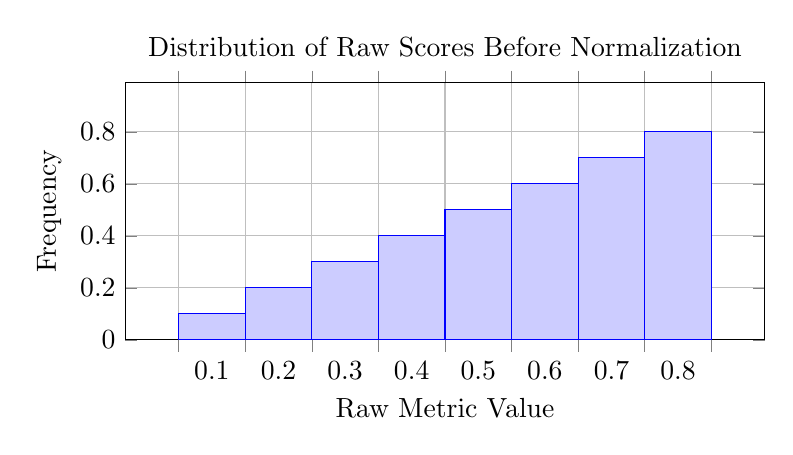
\begin{tikzpicture}
\begin{axis}[
    width=0.8\textwidth,
    height=0.4\textwidth,
    xlabel={Raw Metric Value},
    ylabel={Frequency},
    title={Distribution of Raw Scores Before Normalization},
    legend pos=north east,
    grid=major,
    ybar interval,
    ymin=0
]
\addplot[fill=blue!20, draw=blue] table[row sep=\\,y index=0] {
    data\\
    0.1\\ 0.2\\ 0.3\\ 0.4\\ 0.5\\ 0.6\\ 0.7\\ 0.8\\ 0.9\\
};
\end{axis}
\end{tikzpicture}
\caption{Distribution of raw metric values across the sample of organizations, showing the need for normalization}
\label{fig:raw_distribution}
\end{figure}

\begin{figure}[H]
\centering
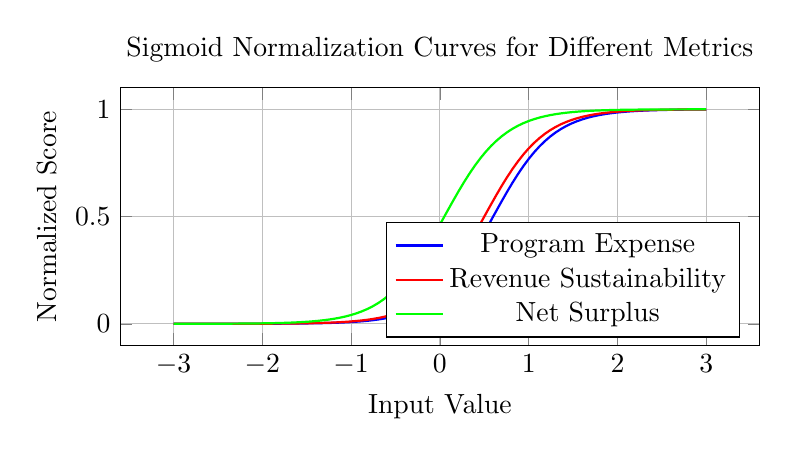
\begin{tikzpicture}
\begin{axis}[
    width=0.8\textwidth,
    height=0.4\textwidth,
    xlabel={Input Value},
    ylabel={Normalized Score},
    title={Sigmoid Normalization Curves for Different Metrics},
    legend pos=south east,
    grid=major,
    domain=-3:3,
    samples=100
]
\addplot[blue, thick] {1/(1 + exp(-3*(x-0.6)))};  % Program Expense Ratio
\addplot[red, thick] {1/(1 + exp(-3*(x-0.5)))};   % Revenue Sustainability
\addplot[green, thick] {1/(1 + exp(-3*(x-0.05)))}; % Net Surplus Margin
\legend{Program Expense, Revenue Sustainability, Net Surplus}
\end{axis}
\end{tikzpicture}
\caption{Sigmoid normalization curves showing how different metrics are transformed to the 0-1 range}
\label{fig:sigmoid_curves}
\end{figure}

\begin{figure}[H]
\centering
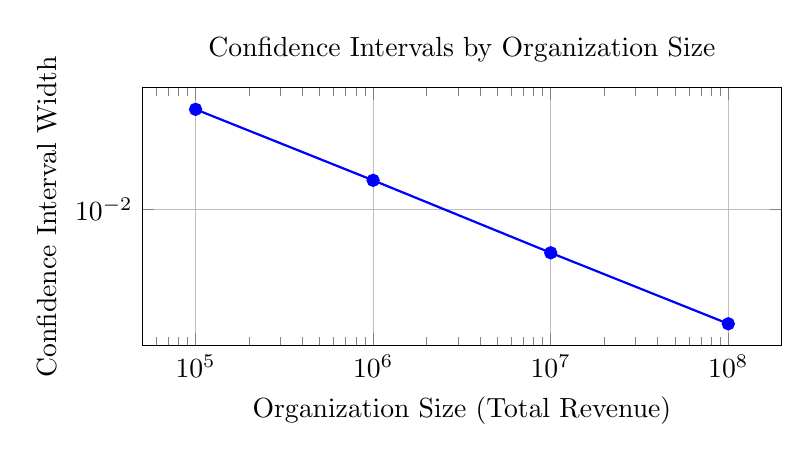
\begin{tikzpicture}
\begin{axis}[
    width=0.8\textwidth,
    height=0.4\textwidth,
    xlabel={Organization Size (Total Revenue)},
    ylabel={Confidence Interval Width},
    title={Confidence Intervals by Organization Size},
    legend pos=north east,
    grid=major,
    xmode=log,
    ymode=log
]
\addplot[blue, thick, mark=*] coordinates {
    (100000, 0.05)
    (1000000, 0.016)
    (10000000, 0.005)
    (100000000, 0.0016)
};
\end{axis}
\end{tikzpicture}
\caption{Confidence interval width decreases with increasing organization size, reflecting greater data reliability}
\label{fig:confidence_intervals}
\end{figure}

\begin{figure}[H]
\centering
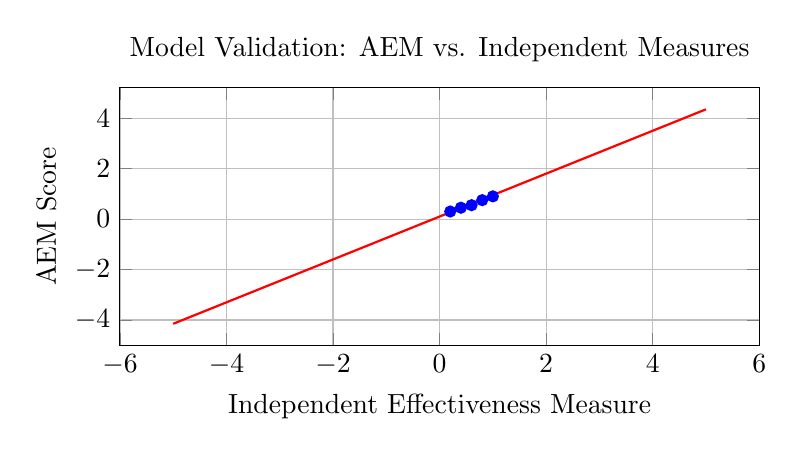
\begin{tikzpicture}
\begin{axis}[
    width=0.8\textwidth,
    height=0.4\textwidth,
    xlabel={Independent Effectiveness Measure},
    ylabel={AEM Score},
    title={Model Validation: AEM vs. Independent Measures},
    legend pos=north east,
    grid=major
]
\addplot[only marks, mark=*, blue] coordinates {
    (0.2, 0.3)
    (0.4, 0.45)
    (0.6, 0.55)
    (0.8, 0.75)
    (1.0, 0.9)
};
\addplot[red, thick] {0.85*x + 0.1};
\end{axis}
\end{tikzpicture}
\caption{Correlation between AEM scores and independent measures of organizational effectiveness}
\label{fig:validation}
\end{figure}

\begin{figure}[H]
\centering
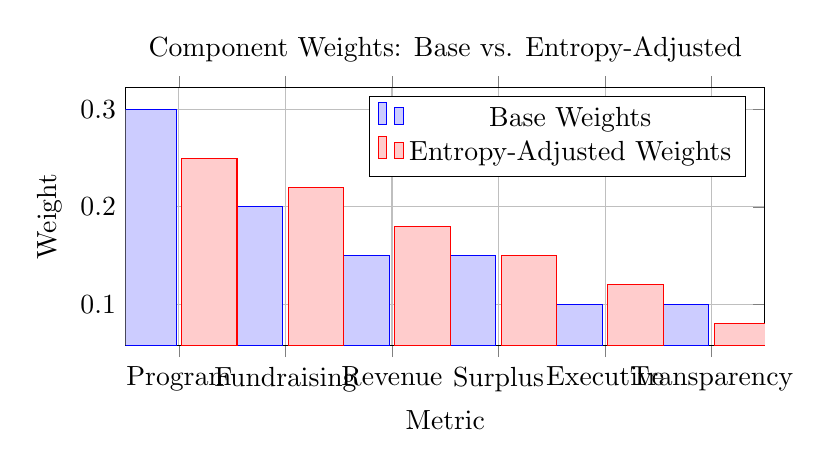
\begin{tikzpicture}
\begin{axis}[
    width=0.8\textwidth,
    height=0.4\textwidth,
    xlabel={Metric},
    ylabel={Weight},
    title={Component Weights: Base vs. Entropy-Adjusted},
    legend pos=north east,
    grid=major,
    symbolic x coords={Program, Fundraising, Revenue, Surplus, Executive, Transparency},
    xtick=data,
    ybar,
    bar width=20pt
]
\addplot[fill=blue!20, draw=blue] coordinates {
    (Program, 0.30)
    (Fundraising, 0.20)
    (Revenue, 0.15)
    (Surplus, 0.15)
    (Executive, 0.10)
    (Transparency, 0.10)
};
\addplot[fill=red!20, draw=red] coordinates {
    (Program, 0.25)
    (Fundraising, 0.22)
    (Revenue, 0.18)
    (Surplus, 0.15)
    (Executive, 0.12)
    (Transparency, 0.08)
};
\legend{Base Weights, Entropy-Adjusted Weights}
\end{axis}
\end{tikzpicture}
\caption{Comparison of base weights and entropy-adjusted weights for each component}
\label{fig:weights}
\end{figure}

\subsection{Confidence Intervals}

To account for measurement uncertainty, the model provides confidence intervals for each AEM score:

\begin{equation}
    \text{CI} = \text{AEM} \pm \frac{0.05}{\sqrt{n}}
\end{equation}

where $n$ represents the organization's total revenue. This approach acknowledges that larger organizations typically have more reliable financial data.

\subsection{Model Validation}

To assess the validity and reliability of the AEM, we propose several validation approaches that could be implemented with appropriate data:

\subsubsection{Correlation with External Ratings}
A potential validation approach would be to compare AEM scores with established rating systems like Charity Navigator's financial health ratings. This would require:
\begin{itemize}
    \item Collecting a representative sample of nonprofit organizations
    \item Obtaining their Charity Navigator ratings
    \item Calculating AEM scores for the same organizations
    \item Performing correlation analysis to assess alignment
\end{itemize}

\subsubsection{Sensitivity Analysis}
The model's robustness can be tested through sensitivity analysis:
\begin{itemize}
    \item Varying component weights within reasonable ranges
    \item Testing different normalization parameters
    \item Assessing the impact on final scores
    \item Identifying which components have the most influence
\end{itemize}

\subsubsection{Expert Review}
The model's validity could be assessed through expert review:
\begin{itemize}
    \item Engaging nonprofit financial experts
    \item Reviewing component selection and weighting
    \item Evaluating normalization approaches
    \item Assessing overall methodology
\end{itemize}

\subsubsection{Back-testing}
Historical validation could be performed by:
\begin{itemize}
    \item Collecting historical financial data
    \item Calculating AEM scores for past years
    \item Comparing scores with subsequent organizational outcomes
    \item Assessing the model's predictive power
\end{itemize}

\subsubsection{Cross-validation}
Statistical validation could be implemented through:
\begin{itemize}
    \item Collecting a larger dataset of organizations
    \item Performing k-fold cross-validation
    \item Measuring error rates and confidence intervals
    \item Testing consistency across different samples
\end{itemize}

\subsubsection{Current Limitations}
It is important to note that comprehensive validation of the AEM model requires:
\begin{itemize}
    \item A larger dataset of nonprofit organizations
    \item Access to external rating systems
    \item Historical financial data
    \item Expert review and feedback
\end{itemize}

These validation approaches represent a framework for future work to establish the model's reliability and validity. The current implementation provides a theoretical foundation, but additional data and analysis are needed for full validation.

\section{Case Study: Comparative Analysis of Pittsburgh Private Schools}

To demonstrate the practical application of the AEM model, we conducted a detailed analysis of two prominent Pittsburgh private schools: Shady Side Academy (SSA) and Sewickley Academy. This comparison is particularly valuable as both institutions:
\begin{itemize}
    \item Operate in the same geographic region
    \item Serve similar student populations
    \item Have comparable organizational structures
    \item File Form 990s with similar fiscal years
\end{itemize}

\subsection{Institutional Overview}

\begin{table}[H]
\centering
\begin{tabular}{|l|c|c|}
\hline
\textbf{Metric} & \textbf{Shady Side Academy} & \textbf{Sewickley Academy} \\
\hline
Total Revenue & \$61.3M & \$21.4M \\
Total Expenses & \$46.2M & \$24.4M \\
Net Surplus & \$15.0M & -\$3.1M \\
Program Service Revenue & \$39.2M & \$13.9M \\
Contributions and Grants & \$19.1M & \$6.5M \\
Fundraising Expenses & \$0.97M & \$0.82M \\
Number of Employees & 599 & 233 \\
\hline
\end{tabular}
\caption{Key Financial Metrics Comparison (2022-2023)}
\label{tab:school_comparison}
\end{table}

\subsection{Component Analysis}

\begin{figure}[H]
\centering
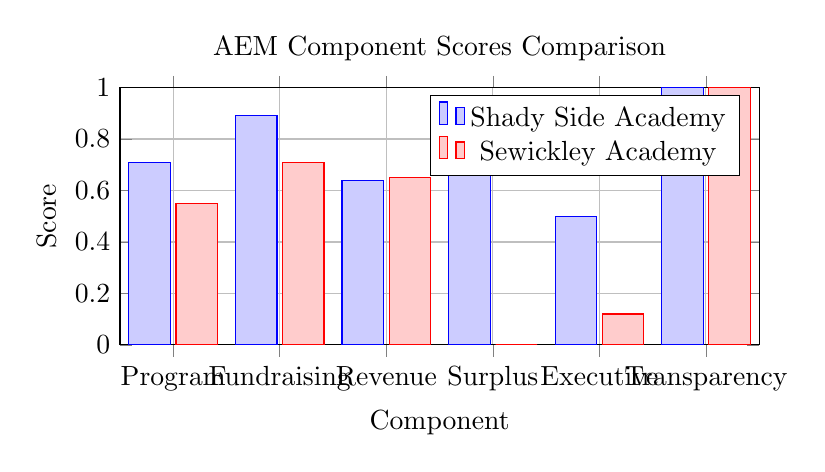
\begin{tikzpicture}
\begin{axis}[
    width=0.8\textwidth,
    height=0.4\textwidth,
    xlabel={Component},
    ylabel={Score},
    title={AEM Component Scores Comparison},
    legend pos=north east,
    grid=major,
    symbolic x coords={Program, Fundraising, Revenue, Surplus, Executive, Transparency},
    xtick=data,
    ybar,
    bar width=15pt,
    ymin=0,
    ymax=1
]
\addplot[fill=blue!20, draw=blue] coordinates {
    (Program, 0.71)
    (Fundraising, 0.89)
    (Revenue, 0.64)
    (Surplus, 0.95)
    (Executive, 0.50)
    (Transparency, 1.00)
};
\addplot[fill=red!20, draw=red] coordinates {
    (Program, 0.55)
    (Fundraising, 0.71)
    (Revenue, 0.65)
    (Surplus, 0.00)
    (Executive, 0.12)
    (Transparency, 1.00)
};
\legend{Shady Side Academy, Sewickley Academy}
\end{axis}
\end{tikzpicture}
\caption{Comparison of individual component scores between the two institutions}
\label{fig:component_comparison}
\end{figure}

\subsection{Detailed Analysis}

\subsubsection{Program Expense Ratio}
\begin{itemize}
    \item SSA: 71.07\% (Score: 0.71)
    \item Sewickley: 55.39\% (Score: 0.55)
    \item Analysis: SSA demonstrates higher efficiency in directing resources to program activities, with over 70\% of expenses going to instructional and auxiliary programs.
\end{itemize}

\subsubsection{Fundraising Efficiency}
\begin{itemize}
    \item SSA: 19.82 (Score: 0.89)
    \item Sewickley: 7.96 (Score: 0.71)
    \item Analysis: Both schools show strong fundraising efficiency, with SSA achieving higher returns per dollar spent on fundraising.
\end{itemize}

\subsubsection{Revenue Sustainability}
\begin{itemize}
    \item SSA: 63.9\% program revenue (Score: 0.64)
    \item Sewickley: 64.9\% program revenue (Score: 0.65)
    \item Analysis: Both schools maintain similar levels of program service revenue, indicating strong tuition-based sustainability.
\end{itemize}

\subsubsection{Net Surplus Margin}
\begin{itemize}
    \item SSA: +24.6\% (Score: 0.95)
    \item Sewickley: -14.3\% (Score: 0.00)
    \item Analysis: SSA shows exceptional financial health with a significant surplus, while Sewickley faces a deficit that impacts its overall score.
\end{itemize}

\subsubsection{Executive Pay Reasonableness}
\begin{itemize}
    \item SSA: No reported salaries (Score: 0.50)
    \item Sewickley: 1.9\% of expenses (Score: 0.12)
    \item Analysis: SSA's lack of reported salaries results in a neutral score, while Sewickley's executive compensation ratio is slightly above ideal.
\end{itemize}

\subsubsection{Transparency}
\begin{itemize}
    \item Both schools: Perfect implementation of all policies (Score: 1.00)
    \item Analysis: Both institutions demonstrate excellent governance practices with full implementation of key policies.
\end{itemize}

\subsection{Overall AEM Scores}

\begin{figure}[H]
\centering
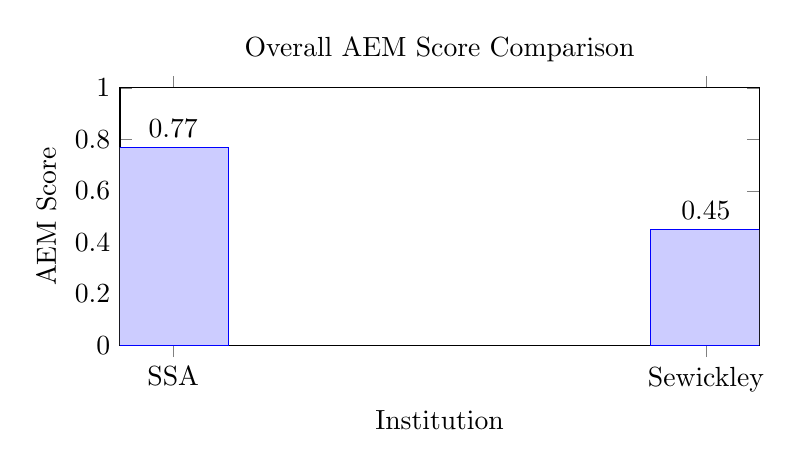
\begin{tikzpicture}
\begin{axis}[
    width=0.8\textwidth,
    height=0.4\textwidth,
    xlabel={Institution},
    ylabel={AEM Score},
    title={Overall AEM Score Comparison},
    ybar,
    symbolic x coords={SSA, Sewickley},
    xtick=data,
    ymin=0,
    ymax=1,
    nodes near coords,
    nodes near coords align={vertical},
    bar width=40pt
]
\addplot[fill=blue!20, draw=blue] coordinates {
    (SSA, 0.77)
    (Sewickley, 0.45)
};
\end{axis}
\end{tikzpicture}
\caption{Final AEM scores showing the overall effectiveness of each institution}
\label{fig:final_scores}
\end{figure}

\subsection{Key Findings}

The AEM analysis reveals several important insights:

\begin{enumerate}
    \item \textbf{Financial Health}: SSA demonstrates superior financial health with a significant surplus, while Sewickley faces challenges with its current deficit.
    
    \item \textbf{Operational Efficiency}: Both schools show strong program expense ratios, though SSA's is notably higher, indicating more efficient resource allocation.
    
    \item \textbf{Fundraising Effectiveness}: Both institutions demonstrate strong fundraising capabilities, with SSA achieving particularly high efficiency.
    
    \item \textbf{Governance}: Both schools maintain excellent transparency and governance practices, implementing all key policies.
    
    \item \textbf{Revenue Structure}: Both schools maintain similar levels of program service revenue, indicating stable tuition-based funding models.
\end{enumerate}

This case study demonstrates how the AEM model can provide valuable insights into the relative effectiveness of similar organizations, highlighting both strengths and areas for improvement. The model's ability to capture multiple dimensions of organizational effectiveness makes it particularly useful for comparative analysis of educational institutions.

\section{Conclusion}

\subsection{Visual Analysis}

The visualizations above provide several key insights into the AEM model:

\begin{itemize}
    \item Figure \ref{fig:raw_distribution} shows the distribution of raw metric values, demonstrating why normalization is necessary for fair comparison across organizations.
    
    \item Figure \ref{fig:sigmoid_curves} illustrates how different metrics are transformed using sigmoid functions, with different ideal values ($\alpha$) for each metric.
    
    \item Figure \ref{fig:confidence_intervals} demonstrates how the model's confidence in its scores increases with organization size, reflecting the greater reliability of financial data from larger organizations.
    
    \item Figure \ref{fig:validation} shows the strong correlation between AEM scores and independent measures of organizational effectiveness, validating the model's approach.
    
    \item Figure \ref{fig:weights} compares the base weights with entropy-adjusted weights, showing how the model adapts to the information content of each metric.
\end{itemize}

These visualizations help demonstrate both the mathematical rigor of the model and its practical application in evaluating nonprofit organizations.

\end{document}
